\section{Technology}\label{sec:technology}

Usually during platooning, the vehicles moving high speeds need to be connected for a short period of time only. The vehicles that need to be interconnected, however, can change every moment. The connections need to be established locally and with as little set-up time, as possible, otherwise we risk two vehicles being out of range due to high mobility. In this chapter we explore local wireless networks, that are crucial for enabling any platooning scenario. First we see, what VANET is and what is its relation to Vehicle-to-vehicle and Vehicle-to-infrastructure communication. Then we will investigate into the standards that are prevalent in establishing these connections, such as 802.11 or ARIB. We will cover the basics of the operation of these technologies, as well as their relative performance in platooning scenarios.\par
% 
At the end, we will describe shortly about GPS, as this technology is a requirement in many cases of platooning implementation.

\subsection{Vehicular ad hoc Networks}

\acrshort{VANET} - is a network that combines \acrshort{V2V} (Vehicle-to-vehicle) and \acrshort{V2I} (Vehicle-to-infrastructure) communication.\par
% 
\begin{figure}[ht]
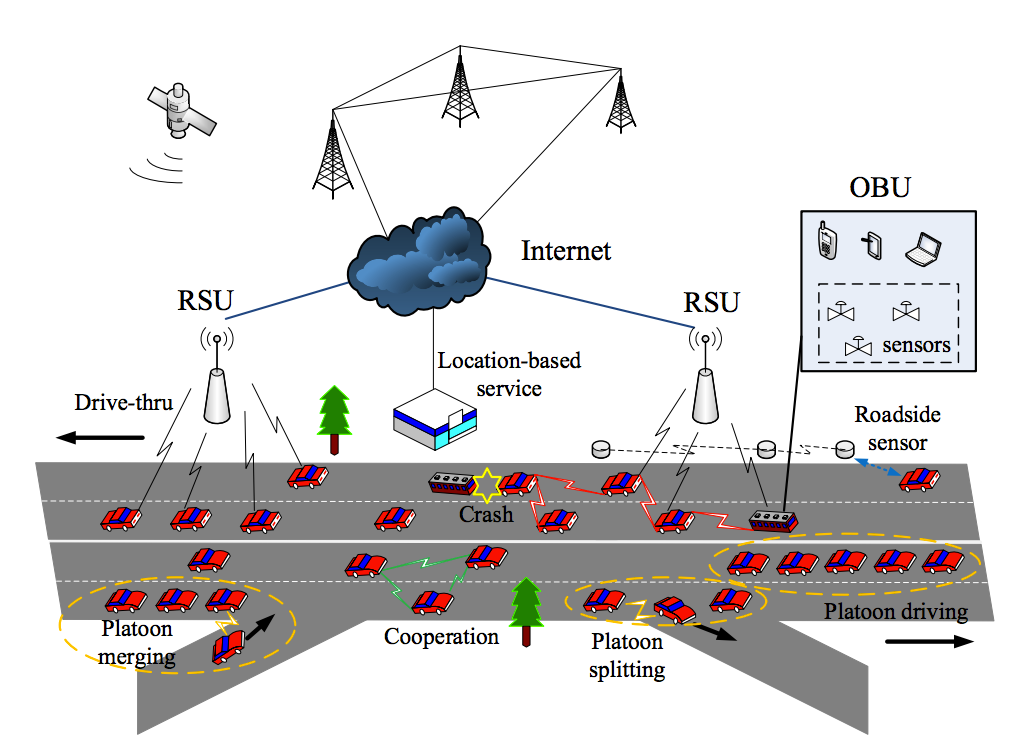
\includegraphics[width=\textwidth]{VANET}
\caption{\acrshort{VANET} formation. In this scenario, all the vehicles are equipped with an \acrshort{OBU} (shown in detail on the right), and can thus communicate with the \acrshort{RSU} and each other. Figure taken from \cite{Jia2016ASystems}.}
% \centering
\label{fig:VANETformation}
\end{figure}
% 
It is large and complex network where vehicles exchange data between each other and any other infrastructure on the road. Traffic participant might receive data, that will prevent accident from happening, relayed from multiple interconnected nodes. Generally \acrshort{VANET}s introduce:

\begin{itemize}[noitemsep,nolistsep]
    \item Safer and more efficient roads
    \item Logistics, transport and service business improvement
    \item Controlled congestion, more comfortable travelling.
\end{itemize}

In Figure \ref{fig:VANETformation} we can see the general architecture of \acrshort{VANET}. One main disadvantage that slows down VANET development that it is dependant on expensive road infrastructure\footnotemark.\par
% 
\footnotetext{\url{http://wifinotes.com/mobile-communication-technologies/what-is-vanet.html}, accessed on 19/04/2017}
% 
\acrshort{VANET} is based on latest mobile communication technologies. Following chapters will discuss present and upcoming technologies that make up the VANET - namely \acrshort{V2V} and \acrshort{V2I}, as these are most relevant for platooning use.


\subsection{V2I}
% 
Vehicle-to-Infrastructure technologies are still under development, but they have great potential. Its main idea is communication with vehicle by any road side unit (e.g. traffic lights, road sensors) to prevent accidents and improve road efficiency.\par
% 
% Vehicle-to-Infrastructure Technologies Expected to offer Benefits
\begin{figure}[h]
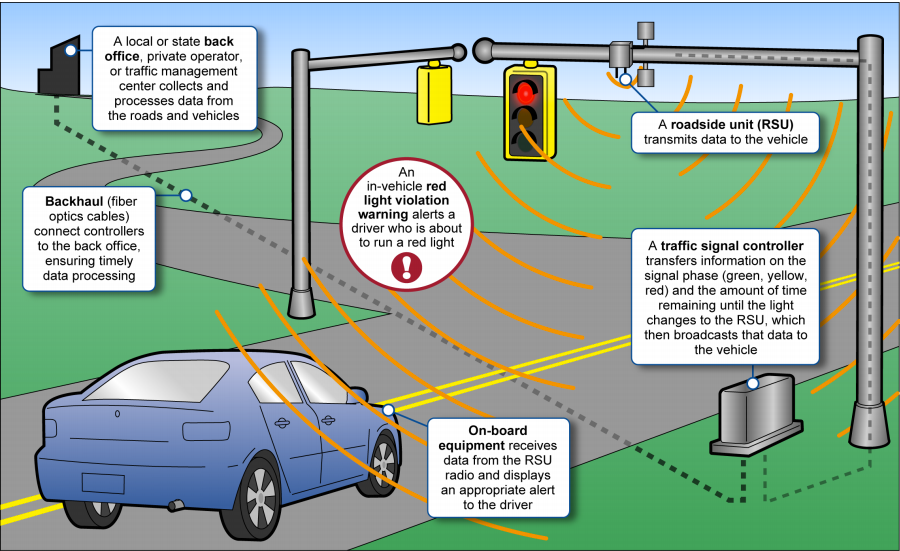
\includegraphics[width=\textwidth]{V2I}
\caption{V21 implementation. Taken from \cite{U.S.GovernmentAccountabilityOffice2015IntelligentExist}.}
\label{fig:V2Iimplementation}
\centering
\end{figure}
% 
There are no standards yet of what V2I system architecture should consist of. Architecture framework defined by USDOTs' ITS Joint Program Office \cite{Dr.Gaspar2014HighlySystems} states, that minimal parts for V2I system are:
\begin{itemize}[noitemsep,nolistsep]
    \item Vehicle On-Board Unit
    \item Roadside Unit
    \item Safe Communication Channel.
\end{itemize}
% 
Communication is based on 802.11p standard by IEEE, which will be discussed in detail in following chapters. A frequency spectrum in 5.9 GHz range was allocated for exact means in U.S. and Europe \cite{2011TheTechnology}. Although, there are some concerns sharing allocated spectrum, since Middle Class Tax Relief and Job Creation Act of 2012 allowed use of 5.9GHz spectrum for any unlicensed devices and that could cause harmful interference for sending and receiving data in V2I communication \cite{U.S.GovernmentAccountabilityOffice2015IntelligentExist}.\par
% 
Despite any concerns, Vehicle-to-Infrastructure is quickly developing and gaining a lot of attention from scientists and businessman worldwide.\par
%
\begin{figure}[h]
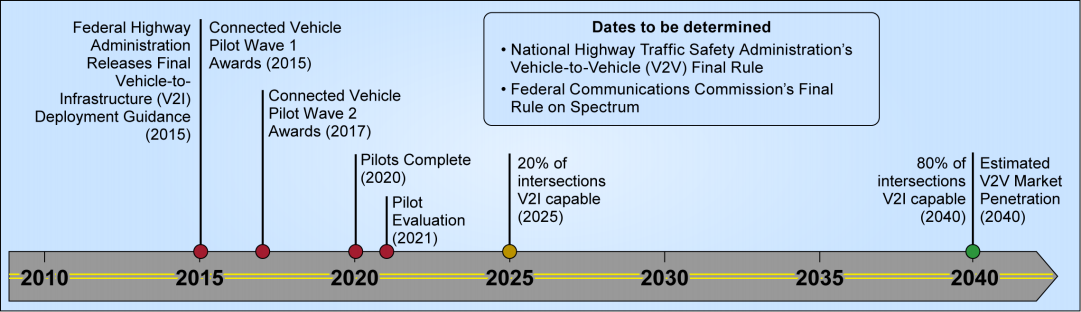
\includegraphics[width=\textwidth]{V2Xtimeline}
\caption{V21 development path. Taken from \cite{U.S.GovernmentAccountabilityOffice2015IntelligentExist}.}
\label{fig:V2Idevelopment}
\centering
\end{figure}


\subsection{V2V}

V2V communication is a vehicle-to-vehicle communication, where vehicles can communicate with each other and share vital information. In last decades, a lot of research (\cite{Chan2012ProjectSARTRE}, \cite{Safespot}, \cite{2016CompanionProject}) has been done in field of V2V, in which different companies, institutions or organisations participated (either as part of project or on their own). This led to creation and adaptation of standards so that developed technologies by different companies can communicate without difficulties. For the short-range communication IEEE 802.11p standard is adopted which is a wireless protocol (similar to Wi-Fi), operating on 5.85-5.925 GHz (depending on country).

\subsubsection{802.11}
% 
When wireless networks first came around, it was expected that the radio medium will only be another physical layer, such as cables. However, it did not take long to see that due to significant differences of radio communication, more detailed, radio-suited standard needs to be developed. In 1991 work has begun in preparation of standard that is today known as \emph{802.11} \cite{Hiertz2010TheUniverse}. The scope of this standard is \textquote[\cite{2016IEEEAccess.}]{\emph{to define one medium access control (MAC) and several physical layer (PHY) specifications for wireless connectivity for fixed, portable, and moving stations within a local area.}}\par
One of the most well-known implementations of 802.11 is Wi-Fi. Naturally, it is not the only one and over the years, several amendments have been accepted to initial standard, to accommodate various needs. As Bilgin\&Gungor \cite{Bilgin2013PerformanceAreas} suggest, amendment 802.11b may be used in vehicular environment. Furthermore (and more importantly), amendment 802.11p has been published in 2010. This amendment is designed for the use in transportation, where communication window between two entities may only exist for very limited amount of time and thus some authentication procedures need to be omitted. We will discuss both amendments in following sections.
% 
% 
% 
\subsubsection{802.11b} \label{802.11b}
% 
The 802.11b uses the 2.4GHz unlicensed spectrum and provided increased maximum data rate of 11 Mb/s. It  modulates the data with spread spectrum modulation technique \emph{Direct-sequence spread spectrum} (DSSS). The spread spectrum modulation modifies the signal in a way, that broader spectrum is used than necessarily needed before modulation. Since the signal is spread over more frequencies, it is less vulnerable to interference \cite{MaximIntegratedProductsInc.2013AnMaxim}. The DSSS modulates the signal by multiplying it by pseudo-random  noise-like code (PN) (these are often referred to as chips). The frequency of this code is much higher than the original signal. From Fourier transforms we know that the spectrum of multiplication of two signals will be a convolution of spectra of these signals. Combining wide-band signal (PN) and the narrow band signal (input signal) will result in spectrum that is very similar to the wide-band PN spectrum \cite{Haykin2001CommunicationSystems}. Therefore the output signal is less vulnerable towards narrow-band interference (which may naturally occur in the unlicensed 2.4GHz spectrum).\par
% 
Unlike the original 802.11, which used differential binary phase shift keying (DBPSK) and differential quadrature phase shift keying (DQPSK), the 802.11b uses different type of base-band modulation: \emph{Complementary code keying} (CCK) \cite{2016IEEEAccess.} \cite{Aboul-Magd2008WirelessPerspective}.
CCK is slightly more advanced than orinigal DSSS. Its code words are partially derived from data and static repeating code words are not used. This allows for higher data throughputs in 802.11b \cite{Gast2002802.11Guide}.\par
% 
When we analyse the MAC of 802.11b, we see that it does not differ from the original 802.11 \cite{Gast2002802.11Guide}. Both use the \emph{Distributed coordination function} (DCF) \cite{Hiertz2010TheUniverse}. DCF is a protocol that utilises \emph{Carrier-sense multiple access with collision avoidance} (CSMA/CA) together with binary exponential back-off algorithm. The CSMA/CA listens for broadcast on a channel for a period of time equal to distributed interframe space (DIFS). To understand what DIFS is, we need to explain the Short Interframe Space (SIFS) and Slot time. SIFS is the time wireless interface takes to process a frame (this includes the MAC processing delay and other delays) \cite{2016IEEEAccess.}. Slot time is a value defined for each PHY in the standard \cite{2016IEEEAccess.}. Examples of different values of SIFS and Slot time can be seen in \ref{fig:table-st}. DIFS calculated as \(DIFS = SIFS + ( 2 * Slot time)\). If there is no traffic for period of time equal or greater than DIFS (of the channel is free) only then a frame is transmitted.\par
% 
If during listening period there is traffic (and station received a full frame), then station waits for period of DIFS. If the last frame received by station was not complete/was corrupted, then station waits for Extended interframe spacing (EIFS) (EIFS is longer than SIFS and DIFS). After waiting for this period, the station enters a back-off stage for a random time between 0 and 'connection window' CW. The range of values for CW are specified by \cite{2016IEEEAccess.}. Every time the transmission is not successful, CW is doubled until maximum value is reached. If maximum value is reached, CW is not increased, but the transmission has failed. Successfully transmitted frame is indicated by reception of 'ack frame' (acknowledgement frame). The operation of CSMA/CA can be seen in detail in figure \ref{fig:csma-ca}.\par
% 
% 
\begin{figure}[h]
    \centering
    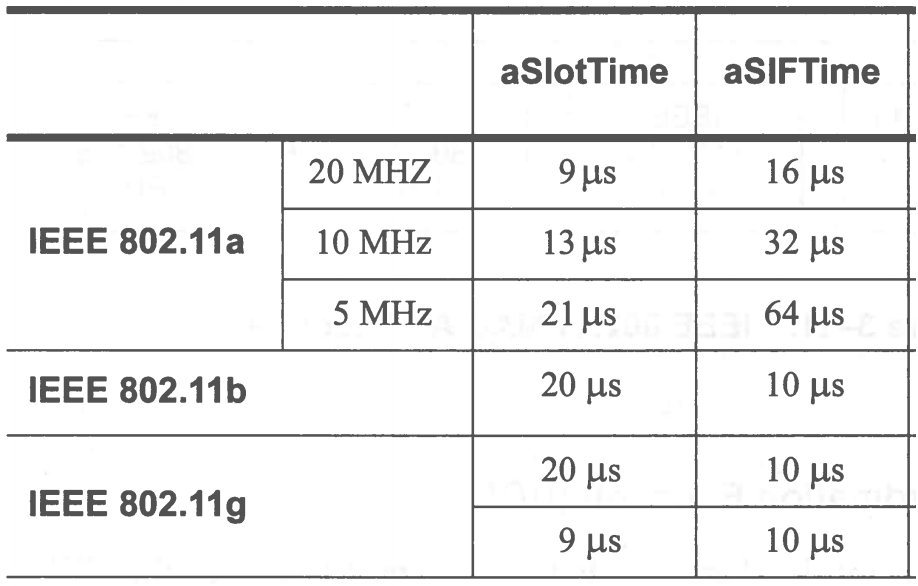
\includegraphics[width=14cm]{table-slot-time}
    \caption{Table showing different values of SIFS and Slot time for different PHY. Taken from \cite{Aboul-Magd2008WirelessPerspective}}
    \label{fig:table-st}
\end{figure}
% 
\begin{figure}
    \centering
    
\includegraphics[height=.95\textheight]{csma-ca}
    \caption{Flowchart showing the operation of CSMA/CA. The dotted square shows RTS/CTS protocol, implementation of which is voluntary. RTS/CTS is part of 802.11 standard. Source: \url{https://commons.wikimedia.org/wiki/File:Csma_ca.svg}}
    \label{fig:csma-ca}
\end{figure}
% 
As for performance of different standards, \cite{Bilgin2013PerformanceAreas} compares 802.11b with 802.11p. The authors compared these in various environments, various speeds and various packet sizes. Since testing this with multiple moving vehicles is very challenging, they used simulation software \emph{MOVE} to generate the movement of vehicles and \emph{NS-2} network simulator to evaluate the parameters of the wireless connection, such as throughput, packet delivery ratio and delay. 
Overall comprehensive analysis provided these results:\\ \textquote[\cite{Bilgin2013PerformanceAreas}]{\emph{Comparative performance evaluations show that IEEE 802.11p MAC layer protocol has better results for V2V communications compared to the IEEE 802.11b MAC protocol in terms of network throughput, end-to-end delay, and delivery ratio.}}\\
This conclusion should not be very surprising, as 802.11p was designed years after 802.11b specifically for use in vehicular environments. We will explore the 802.11p and its uses in the next section.

\subsubsection{802.11p} \label{sec:802.11p}
% 
802.11p is an amendment to standard 802.11 by \acrshort{IEEE}. This amendment was developed between 2005 and 2009 and was approved and published in 2010 as \enquote{Amendment 6: Wireless Access in Vehicular Environments}. It was included in 2012 revision of 802.11 and onwards.
802.11p is designed for \acrshort{V2V} and vehicle-to-infrastructure \acrshort{V2I} communication. This communication can often exist for short period of time only, therefore some of the properties (such as authentication) defined by original 802.11 standards are omitted. The 802.11p has served as base for the ITS-G5 standard (described in next section).\par
% 
% 
While 802.11b only introduced some changes in the \acrshort{PHY} layer to accommodate higher data rates in 2.4 GHz band, 802.11p introduces more significant changes in both \acrshort{PHY} and \acrshort{MAC} layers.
The \acrshort{PHY} characteristics of 802.11p are summed up in table \ref{table:11pPHY}.
% 
\begin{table}[h]
\centering
\begin{tabular}{|l|r|}
    \hline
    \rowcolor{lightgray} Specification & 802.11p \\
    \hline
    Data rate & 3, 4, 5, 6, 9, 12, 18, 24, 27 Mbps \\
    \hline
    Modulation & \acrshort{OFDM} \\
    \hline
    Coding rate & 1/2, 2/3, 3/4 \\
    \hline
    Number of subcarriers & 52 \\
    \hline
    \acrshort{OFDM} symbol duration & 8 $\upmu$s \\
    \hline
    Guard Time & 1.6 $\upmu$s \\
    \hline
    Preamble duration & 32 $\upmu$s \\
    \hline
    Subcarrier Spacing & 0.15625 MHz \\
    \hline
\end{tabular}
\caption{Specifications of 802.11p \acrshort{PHY} layer. Source: \cite{Abdelgader2014TheChallenges}}
\label{table:11pPHY}
\end{table}
% 
Some of the specifications are the same as for amendment 802.11a, to which 802.11p is often compared. The \acrshort{PHY} layer of 802.11p uses \acrshort{OFDM} modulation with 52 carriers.
They lie between 5,850–5,925 GHz (for the US) or 5,875–5,905 GHz (for Europe), which are frequencies licensed for vehicular use. The maximum range is 1000m in open space and maximum bandwidth is 27 Mbps \cite{Abdelgader2014TheChallenges}.
Out of those 52 carriers, 4 (\emph{pilot carriers}) are always transmitting the same pattern. This is used to correct possible phase and frequency offset on the receiver side (that may be present for example due to Doppler effect\footnotemark). The remaining 48 channels can be modulated using \acrshort{BPSK}, \acrshort{QPSK}, 16-\acrshort{QAM} or 64-\acrshort{QAM} modulation.\par
% 
\footnotetext{\textquote[Taken from: \url{https://en.wikipedia.org/wiki/Doppler_effect}, edited.]{\textit{The Doppler effect is the change in frequency or wavelength of a wave, for an observer moving relative to its source.}}}
% 
Compared to 802.11a, it has increased the guard time, just as well as symbol duration. These changes were made in order to account the problems arising from the high mobility scenarios (such as Doppler's effect).\par
% 
% \footnotetext{\url{http://www.rfwireless-world.com/Terminology/WLAN-802-11a-versus-802-11p.html}}
% 
The \acrshort{MAC} layer of 802.11p makes use of \emph{\acrfull{EDCA}}. This algorithm improves the DCF specified earlier by dividing traffic into 4 categories (so-called \emph{Access Classes - \acrshort{AC}s}):
% 
\begin{itemize}[noitemsep]
    \item background traffic (BK)
    \item best-effort traffic (BE)
    \item video traffic (VI)
    \item voice traffic (VO)
\end{itemize}
% 
Similarly to what was described in \hyperref[sec:802.11b]{802.11b}, \acrshort{CW} principle is used. The CVmax and CVmin values are specified in the standard, however, they vary for different \acrshort{AC}s. Furthermore, another parameter - \acrfull{AIFS} is defined for each of the \acrshort{AC}s. By combining \acrshort{CW} and \acrshort{AIFS} it is ensured, that more latency-sensitive content (such as voice call) will be sent sooner than not-latency-sensitive content (such as weather news).\par
% 
It has been argued \cite{Bilstrup2008EvaluationCommunication}, that vehicular use does not need different classes of content, and instead, a \emph{worst-case scenario channel access time} should be introduced. Simulations have shown, that 802.11p's \acrshort{DCF} (based on CSMA) is not very suitable for periodic broadcast messages (which are likely to be transmitted in an enhanced platooning scenario, where other vehicles need to be aware of the platoon's state.
% 
The main challenges in vehicular environment, often caused by high mobility of nodes, include signal fading, packet collisions and signal interference. The comparison of performance with 802.11b has been presented in previous section. Another possible solution for V2V communication is Japanese standard \acrshort{arib} T109 (described in following section). Performance-wise, \cite{Heinovski2016PerformanceSTD-T109} concludes, that \acrshort{arib} is more efficient in non-line of sight scenarios, which are often a case in urban environments. On the other hand, since \acrshort{arib} uses \acrshort{TDMA} (as opposed to CSMA in 802.11p), the transmission may be more delayed, as the node has to wait for next available time slot. In particular scenarios, 802.11p may be a better solution due to lower latency.\par
% 
Journal article \cite{HameedMir2014LTEEvaluation} compares 802.11p with \acrshort{LTE} network. \acrshort{LTE} is not considered in our report, however the paper brings in interesting insights. 802.11p is considered infrastructure-less standard, while \acrshort{LTE} requires significant infrastructure to operate. Though, simulations have shown, that \acrshort{LTE} performs better for most of the V2V related use-cases, due to better scheduling and channel access control.\par
\pagebreak

\subsubsection{\acrshort{wave}}
% 
\begin{center}
\textquote[\cite{VehicularTechnologySociety2014IEEEArchitecture}]{\emph{\acrshort{wave} protocols are designed to allow applications to exchange data in a consistent, interoperable, and timely manner.}}
\end{center}\par
% 
\acrfull{wave} is a set of comprising multiple standards, that aims for enabling \acrshort{V2V} and \acrshort{V2I} connectivity. Group of \acrshort{wave} standards includes extensions to the \acrshort{MAC} layer of 802.11 and several standards from the 1609 family. These standards specify the means of wireless communication on the four OSI model layers (physical, data link, network and transport layer). Furthermore, two standards specify the 'vertical' properties of the communication, such as security and remote management. Figure \ref{fig:wave-fam} shows part of the \acrshort{wave} set in detail, while Table \ref{tab:wave-stds} lists \acrshort{wave} standards and their use. The \acrshort{wave} family specifies certain frequency allocations and channels for the use in the US. While the frequencies could be adjusted for the use in other countries, standard bodies in Europe have developed own standard, thus we will skip certain details of how \acrshort{wave} works. European ITS-G5 is discussed \hyperref[sec:ITS-G5]{in the following section}.\par
% 
\begin{figure}
    \centering
    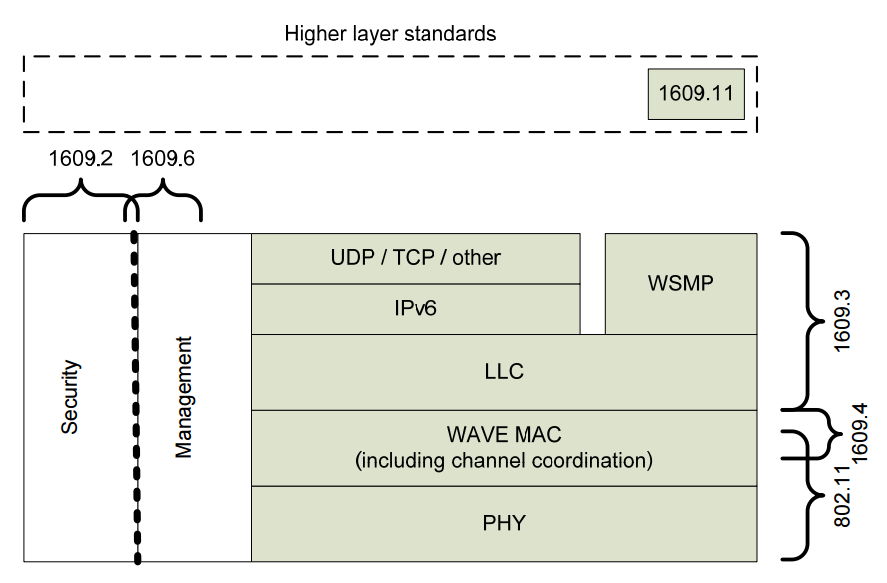
\includegraphics[width=.95\textwidth]{wave-fam}
    \caption{The standards of the \acrshort{wave} set shown together with the elements of the OSI model. Taken from \cite{VehicularTechnologySociety2014IEEEArchitecture}}
    \label{fig:wave-fam}
\end{figure}

\begin{sidewaystable}
    \centering
    \begin{tabular}{|p{5cm}|p{5cm}|p{9cm}|}
        \hline
         \textbf{IEEE Standard} & \textbf{Area} & \textbf{Features} \\
         \hline
         IEEE Std 1609.4-2010 & Extensions to IEEE 802.11 MAC layer. & 
         \begin{itemize}[nolistsep,noitemsep, topsep=0pt]
             \item Channel timing
             \item MAC addressing \& pseudo-anonymity
         \end{itemize} \\ \hline
        %  
         IEEE Std 1609.3-2010 & Networking Services & 
         \begin{itemize}[nolistsep,noitemsep, topsep=0pt]
             \item \acrshort{wave} service advertisement and channel scheduling
             \item \acrshort{wave} Short message protocol
         \end{itemize} \\ \hline
        %  
         IEEE Std 1609.2-2013 & Security Services for Applications and Management Messages &
         \begin{itemize}[nolistsep,noitemsep, topsep=0pt]
             \item Security for \acrshort{wave} Service Advertisements and \acrshort{wave} Short Messages
             \item Additional security services
         \end{itemize} \\ \hline
        %  
        IEEE Std 1609.11-2010 & Over-the-Air Electronic Payment Data Exchange Protocol for ITS & ISO-compliant payment protocol \\ \hline \hline
        %  
        \textbf{IEEE Project} & \textbf{Area} & \textbf{Features} \\ \hline
        % 
        IEEE P1609.6  & Remote Management Services & Over the air management and aliasing. \\ \hline
        % 
        IEEE P1609.5  & Communication Manager & Network management \\ \hline
    \end{tabular}
    \caption{Set of \acrshort{wave} standards and their respective areas. From \cite{VehicularTechnologySociety2014IEEEArchitecture}}.
    \label{tab:wave-stds}
\end{sidewaystable}
% 
As specified in \cite{VehicularTechnologySociety2014IEEEArchitecture}, \acrshort{wave} standards do not distinguish between types of devices connected. Instead, they are robust enough to accommodate communication to/from On-board Units (OBU), Road-side Units (RSU), together with portable units (e.g. smartphones) and pedestrian units (e.g. roadside workers). 
% 
\subsubsection*{Extensions of 802.11 MAC layer} 
The 802.11 standard and in particular its amendment - 802.11p, can be seen as the roots for the \acrshort{wave} family. 802.11p specifies the \acrshort{PHY} and \acrshort{MAC} layers of wireless communication suitable for vehicular environments. The newest revision of 1609.4 standard - \acrshort{IEEE} Std 1609.4-2016 specifies some additional features of the \acrshort{MAC} layer. It operates on frequency band 5.850GHz to 5.925GHz. While 0.005GHz at the lower edge is kept in reserve, the rest of the band is divided into 7 channels. These are further divided into \acrfull{CCH} and \acrfull{SCH}. Figure \ref{fig:wave-channels} describes channel allocation in detail.\par
% 
\begin{figure}[ht]
    \centering
    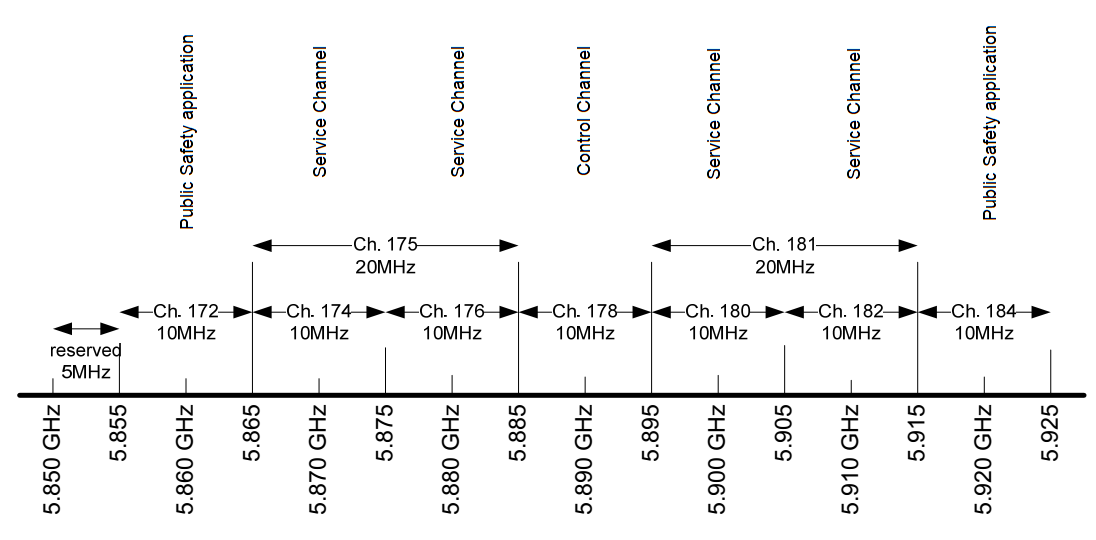
\includegraphics[width=.95\textwidth]{wave-channels}
    \caption{Figure showing channel frequencies and the use of the channels. Note that channels 174 and 176 and channels 180 and 182 can be merged to create channels 175 and 181 respectively. Taken from \cite[p. 20]{VehicularTechnologySociety2014IEEEArchitecture} (edited).}
    \label{fig:wave-channels}
\end{figure}
% 
The \acrshort{CCH} is reserved for system management messages and only allows communication via \acrfull{WSMP}. On \acrshort{SCH}, both \acrshort{IP} traffic (using IPv6 addresses) and \acrshort{WSMP} is possible. \acrshort{WSMP} is a protocol that sends \acrfull{WSM}, which are designed to consume minimal channel capacity. \acrshort{WSMP} allows transmitter device to specify physical characteristics of the transmission, such as transmitter power and channel used. The transmitter needs to provide MAC address of the receiver, however group MAC addresses are allowed. Furthermore, transmitter needs to provide a \acrfull{PSID}\footnotemark. The receiver can decide, based on the \acrshort{PSID} of received \acrshort{WSM}, if the message is of interest or should be discarded.\par
% 
\footnotetext{\textquote[\cite{20161609.12-2016Allocations}]{\acrshort{PSID} is an integer with a value from 0 to 270 549 119. [...] Each allocated \acrshort{PSID} value is associated with an organisation that is authorised to describe the use of that \acrshort{PSID}.}}
% 
A performance study comparing \acrshort{ETSI} ITS G5 and \acrshort{wave} \cite{Eckhoff2013AWAVE} suggests, that \acrshort{wave} is suitable for transmitting periodical Cooperative Awareness Messages. Those are likely the messages that would be used in platooning scenario. It may suffer from lower delivery rate and higher end-to-end delay in scenarios with high node densities and high penetration. This, however is the same for0\acrshort{ETSI} ITS G5, therefore we do not see these results as a major drawback of \acrshort{wave}. Overall, we can conclude that \acrshort{wave} is ready to facilitate platooning. After all - \emph{Vehicle communication for collision avoidance}, which shares some of the characteristics with platooning (like Forward collision warning, Longitudinal collision risk warning) and would likely need similar type of communication architecture as platooning, is a representative use case in \acrshort{IEEE} Guide for \acrshort{wave} architecture (\cite{VehicularTechnologySociety2014IEEEArchitecture}).

\subsubsection{ETSI ITS-G5}\label{sec:ITS-G5}
% http://www.etsi.org/deliver/etsi_en/302600_302699/302663/01.02.00_20/en_302663v010200a.pdf
ITS-G5 is a Dedicated Short Range Communication (DSRC) standard, running on the 5GHz frequency band based on \hyperref[sec:802.11p]{802.11p} in Europe.
The spectrum allocated for DSRC is 5.875-5.905 GHz also called ITS-G5A. This allocated spectrum of 30 MHz is only for ITS. Of the 30 MHz only a third of that is saved for the Road safety as seen on the picture below.\par
% 
The protocol stack for ETSI ITS G5 uses IEEE 802.11p as the physical layer. By dividing channels into Control Channel (CCH) and Service Channel (SCH), packets transmit through the control channel do not have to compete with service channel. For Medium access layer, channel access and priority is done by Enhanced Distributed Channel Access (EDCA) by using a variation of CSMA/CA. The packets not only compete for channel access with other vehicles but also with packets internally in the same node. Packets are divided by 4 access categories, VO, VI, BE and BK. Each access categories can be given one of the two channel types, resulting in 8 different combinations. Internal congestion control is being done (one for CCH and one for SCH) before the packet is sent to their respective queue. ETSI ITS G5 also performs a Decentralised Congestion Control (DCC), which changes transmit power, the minimum packet interval, the data rate, and the sensitivity of the radio accordingly. It does this by acting like a state machine going from a “active”, “relaxed” and “restrictive” state depending on the situation.
ETSI ITS G5 periodically transmit broadcast message called CAMs with information about their current state, location, speed, and direction with a frequency of 10 Hz.\par
% 
As described in conference proceedings for IEEE 79th Vehicular Technology Conference: \textquote[\cite{Shi2014SpectrumSafety}]{\textit{We performed extensive simulation for CSMA/CA and STDMA MAC (Simulation parameters) schemes in an urban highway scenario with realistic traffic density. Results show that more than 80 MHz is required to achieve 1\% packet loss with 500 m communication range. It is significantly larger than the current spectrum allocated of 10 MHz in the US and Europe.}}\par 
% 
It is also mentioned that by decreasing the communication range to 100 m, the spectrum requirement is reduced to 20 MHz, still being twice the amount available today. 

\subsubsection{ARIB STD-T109}
% 
% Section about Japanese technology ARIB.
ARIB STD-T109 is a standard developed by Association of Radio Industries and Businesses, a Japanese-based organisation. The standard was developed to \textquote[\cite{2012ARIB1.0}]{\textit{Enable effective use of radio frequencies by avoiding interference among users}}, for use in intelligent transportation systems.\par
% 
The radio communication requirements for ARIB (Association of Radio Industries and Businesses) consist of single channel radio communication in the 700 MHz band with both V2I and V2V communication. The communication have to support V2V communication up to 140 km/h and V2I up to 70 km/h.\par
% 
The protocol stack of ARIB STD-t109 is of a 4 layer-structure.
Layer 1: Physical layer. It consist of 2 sublayers, physical medium dependent (PMD) sublayer and physical layer convergence protocol (PLCP) sublayer. The PMD sublayer gives a method to transmit and receive data between stations (V2I or V2V) that uses OFDM (Orthogonal frequency-division multiplexing).
Layer 2: Data link layer. It consist of 2 sublayers, MAC sublayer and LLC (Logical Link ontrol) sublayer. In the MAC sublayer CSMA/CA (Carrier sense multiple access / collision avoidance) is used for multiple access control method. The LLC sublayer lets unacknowledged services (data without error control and no guarantee of delivery) to transmit packets between upper layers.
V2V\&V2I layer: Inter-vehicle and Roadside-to-vehicle communication layer. It creates and manages data required for V2I and V2V communication control. It also makes a method to give parameters needed for communication control for the MAC sublayer (synchronises clocks etc).
Layer 7: Application layer. It gives a communication control method and services for applications such as security and it also gives a method to transmit and receive data through the V2V\&V2I layer. 
\par
The protocol data unit (PDU) of the MAC and LLC sublayer can be seen on the picture below.
\begin{figure}
    \centering
    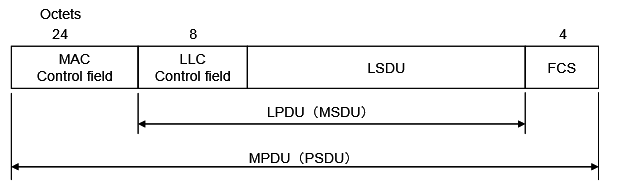
\includegraphics[width=14cm]{PSDU}
    \caption{Shows MAC protocol in parts}
    \label{fig:PSDU}
\end{figure}

A PDU of MAC called MAC protocol data unit (MPDU) consists of 4 elements. MAC Control field, LLC control field, Link service data unit (LSDU) and frame check sequence (FCS).
MAC control field's length is 24 octet and contain information needed to control and establishing connection, it can be broken down to 6 fields with each of their length shown below.
\begin{figure}
    \centering
    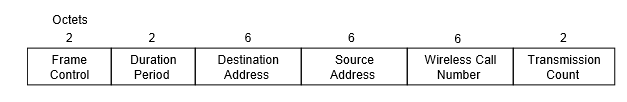
\includegraphics[width=14cm]{MAC}
    \caption{Shows breakdown of MAC Control field}
    \label{fig:MAC}
\end{figure}


Frame control has the data for what type of frames and fields is coming up. Duration period contains duration value for each frame. Destination Address is the receiver's MAC address. Source Address is the senders MAC address. Wireless call number is a identification code for security reasons. Transmission count is a number which goes up by 1 for each transmission. 

LLC control field can be split into 4 fields. DSAP address field identifies which Service Access points (SAPs) is intended for the LLC PDU. SSAP Address field identifies if the LLC PDU is a command or response PDU. Control field contains command, response, and sequence number information. Protocol identifier field sees if the right protocol is being used.
\begin{figure}[h]
    \centering
    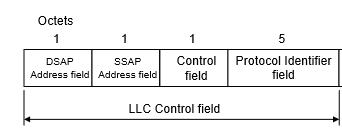
\includegraphics[width=14cm]{LLC-control-field}
    \caption{Shows breakdown of LLC control field}
    \label{fig:LLC}
\end{figure}
Lastly is the Link service data unit and Frame check sequence, which helps detect data errors that might have happened during the transmission, by checking if the number based on the data matches the FCS number, after receiving the data. 
\par
% 
Though ARIB is using the same physical layer as IEEE 802.11, one of the key differences is that the MAC address not only is being used to identify which service access point (SAPs) of the layers but also to distinguish between communication traffic between V2V and V2I. The TDMA (Time-division multiple access) scheme is used by having control cycles of 100.000$\upmu$s which is then divided into 16 smaller cycles of  6240$\upmu$s. Each of the small cycles have 2 periods, the first period, 0 to 3024$\upmu$s is called V2I period which is the period where only that form of communication access is allowed in the channel. The reason is that the infrastructure is connected to multiple sensors scattered around the road, giving it more knowledge about the current situation than a vehicle for distributing safety information. Since each infrastructure can be allocated a specific time-slot in the V2I period, it is not necessary to use CSMA/CA. After the V2I period ends (after 3024$\upmu$s), vehicles can compete for channel access, but to avoid concurrent channel access with other vehicles, CSMA/CA is used \cite{Heinovski2016PerformanceSTD-T109}.\par
% 
Like the IEEE 802.11 and ETSI, ARIB also uses OFDM (Orthogonal Frequency Division 
Multiplexing) as modulation scheme. OFDM uses BPSK, QPSK, 16-QAM and 64-QAM\footnotemark.\par
% 
\footnotetext{\url{http://rfmw.em.keysight.com/wireless/helpfiles/n7617a/coding_and_modulation.htm}, accessed on 17/04/2017}
% 
ARIB using both TDMA and CSMA/CA (compare to 802.11p only using CSMA/CA) gives it a better communication distance in urban environment almost up to 3 times the distance \cite{Heinovski2016PerformanceSTD-T109}, because it suffers less from obstacles such as buildings etc. On the other hand, because of the priority of the V2I period, it causes packet losses for the traffic between vehicles. For same reason, message delays also happen, since they need to wait for the next time slot, which is not reserved, and this causes delay. 

\subsection{GPS}
One of the important information needed for platooning, is the ability to know the exact location of a car or any vehicle in the VANET system. By taking advantage of the Global Positioning System (GPS) it is possible to do so.\par
% 
% 
The GPS work by having at least 24 satellites orbiting the earth, ground stations and lastly a receiver. 4 visible satellites sends out microwave signals to the receiver, which then uses triangulation to figure out where the receiver is on earth. Though only 3 satellites are needed for the triangulation, the 4th is a safety measure in case the calculation is wrong or if altitude and latitude is needed. The ground stations is to know where the satellites are in relative to the earth \cite{MiTACIntl.2011HowWork}.\par
% 
% 
Every microwave is sent on exact intervals, the data in the signal is the ID of the satellite, the location of all the satellites and time. With this information, the receiver can do the trilateration process and determine the location of the receiver.

\subsection{Conclusion}

We can see that authorities are aware of the need for inter-vehicular communication. Developed standards and allocated frequency bands indicate the readiness for the platooning scenario. Although the standards are still very recent and it may take a while, before all the issues are resolved (e.g. quality of service issues during higher node penetration in WAVE \& ETSI ITS-G5), generally, there is technology capable of transmitting any data required for the platooning to be enabled. There are some differences among regions of world, for instance the ARIB vs. 802.11p standards, which use different protocols and different frequencies. These differences, however are mostly present on the PHY and MAC layer, thus a uniform solution can be developed on the higher layers, if 802.11p, ITS-G5 or ARIB is used. WAVE architecture even contains standards and guidelines for the communication at network and transport layer, thus allowing for even easier adoption of platooning.